\documentclass[11pt]{article}
\usepackage[margin=1in]{geometry}
\usepackage{amsmath,amssymb,amsthm,mathtools,bm}
\usepackage{graphicx}
\usepackage{booktabs}
\usepackage[hidelinks]{hyperref}
\usepackage{microtype}
\usepackage{placeins}
\usepackage{tikz}
\usetikzlibrary{arrows.meta,positioning,calc,decorations.pathreplacing,patterns}
\usepackage[numbers,sort&compress]{natbib}

\theoremstyle{plain}
\newtheorem{theorem}{Theorem}
\newtheorem{proposition}{Proposition}
\newtheorem{corollary}{Corollary}
\newtheorem{lemma}{Lemma}
\theoremstyle{definition}
\newtheorem{definition}{Definition}
\newtheorem{assumption}{Assumption}
\newtheorem{remark}{Remark}
\newtheorem{example}{Example}

\newcommand{\Pcal}{\mathcal{P}}
\newcommand{\Gcal}{\mathcal{G}}
\newcommand{\Rset}{\mathcal{R}}
\newcommand{\Wone}{W_1}
\newcommand{\Dop}{\mathsf{D}}
\newcommand{\Dhat}{\widehat{\mathsf{D}}}
\newcommand{\Pidep}{\Pi_\beta}
\newcommand{\Sbeta}{\mathsf{S}_\beta}
\newcommand{\diam}{\operatorname{diam}}
\newcommand{\R}{\mathbb{R}}
\newcommand{\Prob}{\mathbb{P}}

\title{\textbf{Performative Stability in Signal Discovery:\\
Deployment, Crowding, and the Decay--Revival Cycle}}
\author{%
Alejandro Rodr\'iguez Dom\'inguez\thanks{Department of Quantitative Analysis and Artificial Intelligence, Miralta Finance Bank S.A., Madrid, Spain, and Department of Computer Science, University of Reading, United Kingdom. Email: \texttt{arodriguez@miraltabank.com}. Corresponding author.}
\and
Miquel Noguer i Alonso\thanks{Artificial Intelligence Finance Institute, New York, and Courant Institute of Mathematical Sciences, New York University.}}
\date{\today}

\begin{document}
\maketitle

\begin{abstract}
\noindent
A trading signal discovered from market data and then deployed as a rule changes the distribution from which the next signal is estimated. We model this discovery--deployment feedback as a graph-valued self-map that carries a graph to the one re-discovered on the law its own deployment induces, where the deployment scale governs how far the law moves, and a graph is performatively stable when the map returns it unchanged.

Because the admissible graph set is finite, every orbit is eventually periodic. A reachable-set margin replaces the contraction argument used in continuous performative prediction: below a positive deployment scale the update is constant on the reachable set and a unique stable graph is reached in one step; above that scale stable graphs need not exist. In a one-signal deadband model, deployment produces a stable regime, a retention band, and a decay--revival two-cycle. In a linear cross-crowding model, rotations longer than two arise only through off-diagonal crowding within the model.

Public data are used only to examine the two ingredients of the mechanism. Published anomalies decay after publication, and momentum returns reverse where a price-based crowding proxy is high. These patterns are consistent with the mechanism, but they do not identify the graph-level loop or the post-deployment law. A per-strategy test would require observing or instrumenting deployment and estimating the strategy-specific detection margin and impact map.
\end{abstract}

\medskip
\noindent\textit{Keywords:} performative prediction, causal discovery, crowding, alpha decay, fixed points, financial machine learning. \quad \textit{JEL:} C45, C58, G11, G14. \quad \textit{MSC 2020:} 91G15, 37E15, 68T05.

\bigskip

\section{Introduction}\label{sec:intro}

Signal discovery now plays an explicit part in the construction of trading rules, increasingly through methods that read structure rather than mere correlation, including causal discovery. A graph is estimated from historical data, the edges that point into returns are read as exploitable structure, and a portfolio is built to harvest them. This use of discovery differs in one respect from its use in the natural sciences, and the difference is the subject of this paper. The deployment of a discovered graph alters the process that discovery will next confront. A signal that is traded becomes crowded, its edge attenuates, and the law from which the next graph is estimated is no longer the law from which the present graph was estimated. Discovery in markets is therefore not the measurement of a fixed system but one step in a dynamical system whose state includes the analyst.

We formalise that system and describe how it behaves over many rounds. Let $\Dop$ denote the rule that returns a graph from a given market law and the previously held graph, and let $\Pidep$ denote the law that prevails once the rule encoded by a graph is deployed at scale $\beta$. The update $\Sbeta(G)=\Dop(\Pidep(G),G)$ advances a graph through one round of estimation, deployment and re-estimation. A graph is performatively stable when it is a fixed point of this update, that is, when re-estimation on the law its deployment induces returns the same graph. The object is the discovery-level counterpart of the performatively stable model of \citet{perdomo2020}, with a discovered graph in place of a fitted parameter and the deployment scale in place of the sensitivity of the distribution map. The mathematical role of the results is structural. Elementary finite-state arguments expose a feedback mechanism that is obscured in continuous performative-prediction formulations: once discovery outputs graphs rather than parameters, contraction is no longer the natural primitive, and margins on reachable laws determine whether the graph update stabilises or cycles. On a finite graph state space with positive minimal separation, a strict contraction self-map cannot generate nontrivial graph dynamics, since along iterates the distances between distinct states would have to shrink below the minimal positive separation; the relevant primitive is instead the margin separating reachable laws from the discovery switching surfaces.

The word causal is used here in a precise and limited way, and the distinction matters for what follows. Deployment is a causal act: committing capital to the mechanisms a graph marks active is an intervention that changes the joint law of signals and returns, and the crowding that erodes an edge is the effect of that intervention. This is the causal content the paper rests on, and it requires no identification. We do not, separately, claim that the discovery operator recovers a true causal graph from observational data; that would require identifiability conditions we neither assume nor test. The operator may be a constraint-based or score-based causal discovery procedure \citep{spirtes2000, chickering2002} or a thresholded predictive screen, and the results hold for any of them. A reader who prefers to read the graph set as labels for competing trading rules loses none of the argument.

Three statements organise the paper. The first is a fact about finite maps and needs no assumption beyond finiteness of the graph set: the orbit of $\Sbeta$ from any starting graph is eventually periodic, with transient and period bounded by the number of graphs. Eventual periodicity is not convergence, and a fixed point is only one of the possible periods. The second holds under a single regularity condition on the reachable laws, that discovery does not change its output under sufficiently small perturbations there. Under that condition there is a strictly positive deployment scale below which the map is constant, a unique stable graph is reached in one step, and the deployed law is unique on the reachable set. The third is a construction. For a single signal we give the phase diagram under entry and exit thresholds: a stable regime below the exit scale, in which the traded graph is the unique absorbing state, and a cycling regime above it, in which a deployed edge is crowded below detection, the capital withdraws, the edge revives, and the rule re-enters. Inside the stable regime the hysteresis creates a retention band, where a signal already traded is held at a deployment scale at which a signal not yet traded would not be entered, so continuation and re-entry occur at different scales; coexisting stable states require in addition that the off-state not fully reset the edge, which we treat as an extension. We then show that, in a linear cross-crowding model, cycles longer than two require off-diagonal crowding, so a rotation among strategies follows from capacity competition rather than from assumption.

The economic content of these statements is that the post-publication decay of an anomaly and its later revival are not independent events but two phases of one deployment-driven cycle. The same mechanism that erodes a crowded edge restores it once capital leaves, so an apparently dead strategy can be in the trough of a cycle rather than permanently arbitraged away, and the scale of deployed capital, not the passage of time, is what determines which regime a strategy is in. This reframes two facts the empirical literature has treated separately, post-publication attenuation and the reversal of crowded trades, as the down and up phases of the same loop, and it implies that a backtest which re-enters on apparent revival is trading the cycle itself rather than a recovered edge.

The contribution is fourfold. First, we formulate signal discovery and deployment as a finite graph-valued feedback system; the state is not a fitted parameter but the graph that a trading rule treats as active. Second, we replace contraction by a reachable-set margin: finiteness gives eventual periodicity, while the margin determines whether the update is constant, stable, or cyclic. Third, we derive the one-signal entry--exit phase diagram and show how crowding produces decay and revival as two phases of the same loop. Fourth, we show how estimation error affects the population loop away from switching surfaces, and examine public data for ingredient-level consistency. The register is conceptual and financial: the individual finite-state arguments are elementary by design, and the economic content, that post-publication decay and the reversal of crowded trades are phases of one deployment cycle, is the point of the construction. Standard and used only as modelling inputs are the linear and concave price-impact forms and the mean--variance capacity model of Equation~\eqref{eq:capacity}, both stated in full in the body.

The remainder proceeds as follows. Section~\ref{sec:setup} fixes the dynamical system, states the discovery rule together with its margin, and separates the deterministic population operator from the finite-sample estimator used in the experiments. Section~\ref{sec:theory} proves the results and treats the boundary cases that the construction requires. Section~\ref{sec:finitesample} gives the high-probability bound under which the estimated loop tracks the population loop. Section~\ref{sec:experiments} reports the Monte Carlo validation, including a robustness battery and confidence bands. Section~\ref{sec:empirical} examines the two ingredients of the mechanism on published anomalies and on a return-based crowding measure, and sets out what a per-strategy diagnostic would additionally require. Section~\ref{sec:related} places the work in relation to performative prediction, causal discovery and the literature on capacity and crowding.

\section{The discovery and deployment system}\label{sec:setup}

We work on a space $(\Pcal,\Wone)$ of market laws equipped with the Wasserstein-$1$ metric. The proofs use only that $\Wone$ is a metric, so any metric inducing the same notion of proximity may replace it; the choice of Wasserstein-$1$ is for concreteness and because it is the metric in which deployment sensitivity is most naturally expressed. The set of admissible graphs $\Gcal$ is finite and carries a metric $d_\Gcal$, which enters the analysis only through the minimal separation $m=\min_{G\neq G'}d_\Gcal(G,G')$, which is positive because the set is finite, and through the diameter $\diam(\Gcal)$.

Each admissible graph has as vertices the traded signals and the return, and an edge records a directed mechanism the rule treats as exploitable. Deployment acts on this system rather than relabelling it. Committing capital at scale $\beta$ to the mechanisms $G$ marks active changes the joint law of signals and returns, which in the language of structural causal models is the interventional law $\Pidep(G)=P^{\,\mathrm{do}(a_\beta(G))}$ induced by setting the allocation to the value $a_\beta(G)$ the rule prescribes. The notation $P^{\,\mathrm{do}(a_\beta(G))}$ is structural-model notation for the post-deployment law specified by the model; it is not an empirical identification claim. In Section~\ref{sec:empirical}, publication and comomentum are used as observable proxies for deployment pressure, and they do not identify $\Pidep(G)$, the allocation intervention $a_\beta(G)$, or the causal graph behind a signal. The loop is thus a sequence of modelled interventions, each estimated from the law the previous one produced, and stability asks whether a graph is a fixed point of its own interventional consequence. The crowding that erodes an edge is the modelled effect of the allocation on the mechanism the edge records, which is why the construction is about deployment as an intervention and not about recovering structure from observation.

\begin{definition}\label{def:loop}
A population discovery operator is a map $\Dop:\Pcal\times\Gcal\to\Gcal$ that returns a new graph from the current law and the previously held graph, the second argument resolving any region in which the law alone does not determine the call. For each deployment scale $\beta\ge0$ a deployment operator $\Pidep:\Gcal\to\Pcal$ returns the interventional law $\Pidep(G)=P^{\,\mathrm{do}(a_\beta(G))}$ that prevails once the rule encoded by $G$ is deployed at scale $\beta$. The state of the system is the current graph, and one round is
\begin{equation}\label{eq:update}
G_{t+1}=\Sbeta(G_t):=\Dop\!\big(\Pidep(G_t),\,G_t\big).
\end{equation}
We write $\Rset_\beta=\{\Pidep(G):G\in\Gcal\}$ for the finite set of reachable deployed laws. A graph $G^\star$ is performatively stable at scale $\beta$ when $\Sbeta(G^\star)=G^\star$.
\end{definition}

Because $\Gcal$ is finite, $\Sbeta$ is still a self-map of a finite set, so the orbit results of Section~\ref{sec:theory} go through unchanged; the second argument of $\Dop$ only enlarges the state from the law to the pair, and the state space remains finite. The history dependence is what lets the discovery rule carry a deadband, the entry--exit hysteresis that a memoryless $\Dop:\Pcal\to\Gcal$ could not represent, and it is what makes the boundary case of the threshold a property of the update rule rather than an ad hoc convention. When discovery does not depend on the previous graph, $\Dop(P,G)=\Dop(P)$ and \eqref{eq:update} reduces to the memoryless loop.

The formulation treats the previous graph as the state variable the discovery rule needs. If residual crowding, capital inertia, delayed impact, or inventory state matters, the state can be enlarged to $\widetilde G_t=(G_t,H_t)$, where $H_t$ records the additional finite or discretised state, and all finite-state results below apply to the enlarged space. The two-graph model is therefore the minimal reset model, not the only admissible state representation.

The operator $\Dop$ is the deterministic object that returns the graph one would obtain from the exact law and the current state. In any application one observes a finite sample from the deployed law and applies an estimated operator $\Dhat_n$, a random map that converges to $\Dop$ in probability as the sample grows whenever the underlying discovery rule is consistent. Every result in Section~\ref{sec:theory} concerns the population operator and is deterministic; Section~\ref{sec:finitesample} gives a high-probability bound under which the estimated loop tracks the population loop, and the experiments of Section~\ref{sec:experiments} use the estimator and therefore test whether the conclusions survive estimation noise. We keep the two objects distinct throughout and never read a property of one as a property of the other.

\begin{figure}[t]
\centering
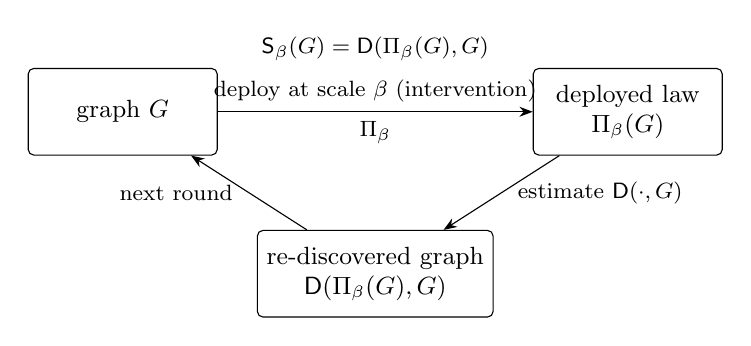
\begin{tikzpicture}[
  >=Stealth, box/.style={draw, rounded corners=2pt, minimum width=24mm, minimum height=11mm, align=center, font=\small},
  lab/.style={font=\footnotesize}]
  \node[box] (G) {graph $G$};
  \node[box, right=40mm of G] (P) {deployed law\\ $\Pi_\beta(G)$};
  \node[box, below=15mm of $(G)!0.5!(P)$] (Gp) {re-discovered graph\\ $\mathsf{D}(\Pi_\beta(G),G)$};
  \draw[->] (G) -- node[lab, above]{deploy at scale $\beta$ (intervention)} node[lab, below]{$\Pi_\beta$} (P);
  \draw[->] (P) -- node[lab, right, align=left]{\;estimate $\mathsf{D}(\cdot,G)$} (Gp);
  \draw[->] (Gp) -- node[lab, left, align=right]{next round\;} (G);
  \node[lab] at ($(G)!0.5!(P)+(0,8mm)$) {$\mathsf{S}_\beta(G)=\mathsf{D}(\Pi_\beta(G),G)$};
\end{tikzpicture}
\caption{One round of the discovery and deployment system. A graph is deployed at scale $\beta$, the deployed rule changes the market law, and the new law is estimated to give the next graph. A graph is performatively stable when this round returns it unchanged.}
\label{fig:loop}
\end{figure}

The first structural assumption is that deployment moves the law continuously from rest. Formally, there is a nondecreasing function $L_\Pi$ with $L_\Pi(\beta)\to0$ as $\beta\to0$ such that $\Wone(\Pidep(G),\Pidep(G'))\le L_\Pi(\beta)\,d_\Gcal(G,G')$ for all graphs $G,G'$.

\begin{assumption}\label{ass:A1}
There exists a nondecreasing $L_\Pi:[0,\infty)\to[0,\infty)$ with $L_\Pi(\beta)\to0$ as $\beta\to0$ such that $\Wone(\Pidep(G),\Pidep(G'))\le L_\Pi(\beta)\,d_\Gcal(G,G')$ for all $G,G'\in\Gcal$.
\end{assumption}

At zero scale no capital is committed, the deployed law does not depend on the graph, and $L_\Pi(0)=0$. The metric $d_\Gcal$ is used only to measure separation among finitely many graph states; since $\Gcal$ is finite, any two metrics inducing the discrete topology are equivalent up to constants, so Assumption~\ref{ass:A1} is not a smoothness condition on graph space but a small-scale deployment condition: as $\beta\downarrow0$, all deployed laws collapse to the no-deployment law uniformly over graphs. The relevant magnitude is the diameter of the reachable set,
\begin{equation}\label{eq:spread}
\Delta(\beta)=\diam(\Rset_\beta)=\sup_{G,G'\in\Gcal}\Wone(\Pidep(G),\Pidep(G'))\le L_\Pi(\beta)\,\diam(\Gcal),
\end{equation}
which we call the deployment spread and which vanishes at $\beta=0$.

The second assumption concerns the discovery operator and is imposed only on the laws the system can reach. On the reachable set, discovery is insensitive to perturbations smaller than a fixed margin, and below the margin the call does not depend on the previous graph.

\begin{assumption}[Reachable-set constant-call margin]\label{ass:A2}
There exists $\rho_\Dop>0$ such that whenever every reachable law lies within $\rho_\Dop$ of a common law, that is $\diam(\Rset_\beta)<\rho_\Dop$, the discovery output is the same for all reachable laws and all previous graphs: there is a single $G^\star\in\Gcal$ with $\Dop(P,G)=G^\star$ for all $P\in\Rset_\beta$ and all $G\in\Gcal$.
\end{assumption}

This is the form the threshold result needs, and it is exactly what the deadband rule delivers when the reachable laws are close enough together. If every reachable edge statistic lies strictly above the entry threshold (or strictly below the exit threshold), then the deadband returns the on-state (respectively the off-state) regardless of the previous graph, because the retain clause is never invoked: the previous graph matters only inside the band, and a spread below the margin keeps the system out of the band on one side. The earlier objection, that a state-dependent rule could retain different graphs even when all laws agree, is therefore ruled out precisely when the reachable laws sit on one side of the band, which is the regime the threshold theorem concerns. A margin, not a contraction, is the appropriate primitive here, for the reason given in the introduction: on a finite graph state space with positive minimal separation a strict contraction cannot generate nontrivial graph dynamics, so the contraction conditions of the parametric performative-prediction literature have no analogue. The margin is imposed only on the reachable set $\Rset_\beta$, not globally on $\Pcal$.

The margin is stated on the law in Wasserstein distance, while the constructions threshold scalar edge statistics, and the two must be connected for the threshold theorem to bind. The following lemma derives the reachable-set constant-call margin of Assumption~\ref{ass:A2} from a primitive condition on the statistics, so that the threshold theorem rests on a statistic margin rather than on an assumed constant call.

\begin{lemma}[Statistic margin implies reachable-set constant call]\label{lem:bridge}
Let discovery evaluate statistics $\phi_j:\Pcal\to\R$ for $j=1,\dots,J$, each $L_j$-Lipschitz on the reachable set in $\Wone$, and write $L_\phi=\max_{1\le j\le J}L_j$. Suppose all reachable statistics lie on the same strict side of their relevant entry or exit thresholds with scalar margin at least $\rho>0$. If
\[
\diam(\Rset_\beta)<\rho/L_\phi,
\]
then discovery returns the same graph for all reachable laws and all previous graphs, so Assumption~\ref{ass:A2} holds with $\rho_\Dop=\rho/L_\phi$.
\end{lemma}

\begin{proof}
For any two reachable laws $P,P'$ and each $j$, Lipschitzness gives $|\phi_j(P)-\phi_j(P')|\le L_j\,\Wone(P,P')\le L_\phi\diam(\Rset_\beta)<\rho$. Since each reachable statistic sits at distance at least $\rho$ from its relevant threshold on a fixed side, a change smaller than $\rho$ cannot move it across, so $\phi_j(P)$ and $\phi_j(P')$ lie on the same side of every threshold. The deadband then returns the same call on every edge regardless of the previous graph, because the retain clause is invoked only inside a band, which no reachable statistic enters. Hence the discovered graph is the same for all reachable laws and all previous graphs.
\end{proof}

The Lipschitz hypothesis is a condition on the edge statistics, not an automatic fact. The mean long-short return is Lipschitz in $\Wone$ when the position weights are bounded, since the spread is then a bounded-Lipschitz functional of the return law; in the constructions we take the traded payoff to be bounded, as it is after the position limits and winsorisation used in any implementation, and $L_\phi$ is the corresponding bound. Without such a condition the bridge does not hold, and the margin would have to be assumed directly in law space. We write the resulting law-space margin as
\begin{equation}\label{eq:bridge}
\rho_\Dop=\rho/L_\phi.
\end{equation}

It remains to fix the discovery rule used in the constructions. Discovery compares an edge statistic $\phi$ to an inclusion threshold $\tau$ with a deadband of half-width $\rho\ge0$, and resolves the band using the previously held graph.

\begin{definition}\label{def:deadband}
The deadband discovery rule with threshold $\tau$ and half-width $\rho\ge0$ sets, for current law $P$ with edge statistic $e=\phi(P)$ and previous graph $G$,
\[
\Dop(P,G)=\begin{cases}
G_{\mathrm{on}}, & e>\tau+\rho,\\
G_{\mathrm{off}}, & e<\tau-\rho,\\
G, & \tau-\rho\le e\le\tau+\rho.
\end{cases}
\]
When $\rho=0$ this is strict thresholding and the dependence on $G$ disappears except on the null set $e=\tau$. With $\rho>0$ the rule has entry--exit hysteresis: an inactive signal becomes active only above $\tau+\rho$ and an active signal turns off only below $\tau-\rho$, so the two switching scales differ and the band depends on the state.
\end{definition}

Through the bridge \eqref{eq:bridge} the deadband half-width $\rho$ on the statistic and the discovery margin $\rho_\Dop=\rho/L_\phi$ on the law are the same quantity in two units. We use $\rho_\Dop$ in the abstract threshold of Section~\ref{sec:theory} and $\rho$ in the constructions and experiments.

The paper works at three levels, and keeping them distinct is essential to reading the claims correctly. Figure~\ref{fig:taxonomy} sets them out: a population loop analysed exactly as finite-state theory, an estimated loop whose finite-sample behaviour is a recovery result away from switching surfaces, and public proxies that supply ingredient-level evidence rather than identification of the loop.

\begin{figure}[t]
\centering
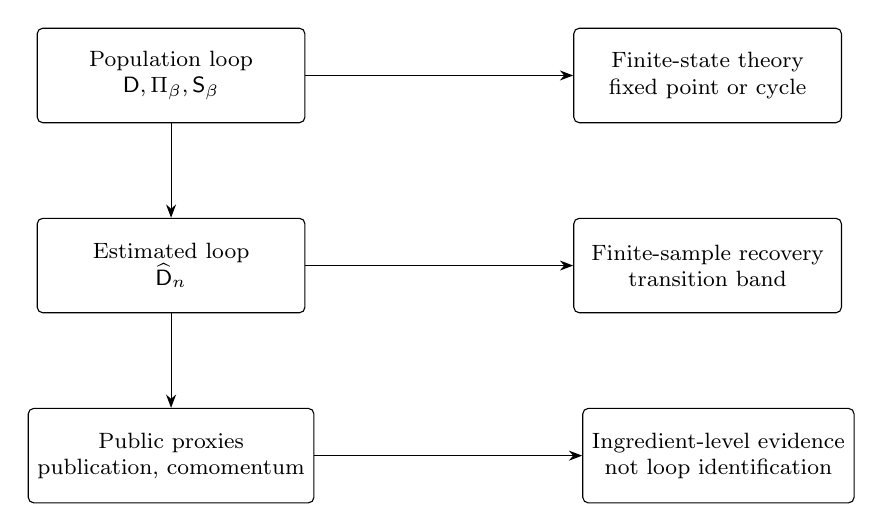
\begin{tikzpicture}[
  >=Stealth, font=\footnotesize,
  box/.style={draw, rounded corners=2pt, align=center, minimum width=34mm, minimum height=12mm},
  lab/.style={font=\scriptsize, align=center}]
  \node[box] (pop) {Population loop\\ $\Dop,\Pidep,\Sbeta$};
  \node[box, right=34mm of pop] (poptheory) {Finite-state theory\\ fixed point or cycle};
  \node[box, below=12mm of pop] (est) {Estimated loop\\ $\Dhat_n$};
  \node[box, right=34mm of est] (esttheory) {Finite-sample recovery\\ transition band};
  \node[box, below=12mm of est] (data) {Public proxies\\ publication, comomentum};
  \node[box, right=34mm of data] (dataev) {Ingredient-level evidence\\ not loop identification};
  \draw[->] (pop) -- (poptheory);
  \draw[->] (est) -- (esttheory);
  \draw[->] (data) -- (dataev);
  \draw[->] (pop) -- (est);
  \draw[->] (est) -- (data);
\end{tikzpicture}
\caption{The three epistemic layers of the paper. The population loop is analysed exactly; the estimated loop is governed by the finite-sample recovery result away from switching surfaces; the public proxies provide consistency evidence for the two ingredients of the mechanism, not identification of the graph-level loop or the post-deployment law.}
\label{fig:taxonomy}
\end{figure}

\section{Stability, threshold, and cycle}\label{sec:theory}

The first result is the elementary fact that drives the existence half of the theory. A deterministic self-map of a finite set has an eventually periodic orbit from every starting point.

\begin{proposition}\label{prop:periodic}
For every $\beta\ge0$ and every $G_0\in\Gcal$ the orbit defined by $G_{k+1}=\Sbeta(G_k)$ is eventually periodic, with transient length and period both at most $|\Gcal|$. The statement does not assert convergence and does not produce a fixed point; a fixed point is the case of period one among the possible periods.
\end{proposition}

\begin{proof}
The map $\Sbeta$ sends the finite set $\Gcal$ to itself, so among the $|\Gcal|+1$ iterates $G_0,\dots,G_{|\Gcal|}$ two must agree. Let $p<q\le|\Gcal|$ be the first pair with $G_p=G_q$ and set $r=q-p$. Determinism gives $G_{k+r}=G_k$ for all $k\ge p$, and both $p$ and $r$ are at most $|\Gcal|$.
\end{proof}

The substantive content lies in which period occurs, and that is governed by the deployment scale through the spread $\Delta(\beta)$. When the spread is smaller than the discovery margin, every reachable law produces the same discovered graph, the map on graphs is constant, and stability is immediate and unique.

\begin{theorem}\label{thm:threshold}
Suppose Assumptions~\ref{ass:A1} and~\ref{ass:A2} hold, and fix a scale $\beta$ with $\Delta(\beta)<\rho_\Dop$. Then there is a graph $G^\star$ such that $\Sbeta(G)=G^\star$ for every $G\in\Gcal$: the update is constant, $G^\star$ is the unique performatively stable graph, and it is reached in one step from any starting graph. The deployed law $P^\star=\Pidep(G^\star)$ is the unique recurrent deployed law after one update: for every starting graph $G$,
\[
\Pidep(\Sbeta(G))=\Pidep(G^\star).
\]
This does not assert that $\Pidep(G)=\Pidep(G^\star)$ for every $G\in\Gcal$; it asserts uniqueness of the deployed law on the recurrent graph state. The conclusion holds for all scales satisfying $L_\Pi(\beta)\diam(\Gcal)<\rho_\Dop$, a set that contains a nonempty interval $[0,\bar\beta)$; no claim is made at boundary scales where equality holds.
\end{theorem}

\begin{proof}
By \eqref{eq:spread}, $\Delta(\beta)=\diam(\Rset_\beta)<\rho_\Dop$, so the hypothesis of Assumption~\ref{ass:A2} is met and there is a single $G^\star$ with $\Dop(P,G)=G^\star$ for all $P\in\Rset_\beta$ and all $G\in\Gcal$. Hence for every graph $G$, the deployed law $\Pidep(G)$ lies in $\Rset_\beta$ and $\Sbeta(G)=\Dop(\Pidep(G),G)=G^\star$, so the update is constant with value $G^\star$. A constant self-map has $G^\star$ as its only fixed point and carries every graph to it in one step. The deployed law after one round is $\Pidep(\Sbeta(G))=\Pidep(G^\star)$ from any start, so $\Pidep(G^\star)$ is the unique recurrent deployed law. For the threshold, $L_\Pi(0)\diam(\Gcal)=0$, and $\beta\mapsto L_\Pi(\beta)\diam(\Gcal)$ is nondecreasing with limit zero at the origin, so the strict inequality $L_\Pi(\beta)\diam(\Gcal)<\rho_\Dop$ holds on a nonempty interval $[0,\bar\beta)$. Since $\Delta(\beta)\le L_\Pi(\beta)\diam(\Gcal)$, every such $\beta$ satisfies the hypothesis.
\end{proof}

The hypothesis is a strict inequality, and equality is left outside the statement. When $\Delta(\beta)$ equals the margin two reachable laws may be exactly the margin apart, a separation at which Assumption~\ref{ass:A2} no longer forces agreement, so the conclusion is asserted only on the open set where the spread is strictly below the margin. The deadband of Definition~\ref{def:deadband} removes the analogous boundary in the cyclic construction that follows.

A local version of the threshold result holds whenever a stable graph exists and discovery is constant on a neighbourhood of its deployed law. It shows that the stable graph attracts an entire ball of graphs in a single step.

\begin{proposition}[One-step basin under local constant discovery]\label{thm:basin}
Suppose $G^\star$ is performatively stable at scale $\beta$, and $\Dop(P,G)=G^\star$ for every law $P$ in the ball $B(\Pidep(G^\star),\rho)$ and every previous graph $G$, for some $\rho>0$. If a set $\mathcal B\subseteq\Gcal$ satisfies $L_\Pi(\beta)\,d_\Gcal(G,G^\star)<\rho$ for every $G\in\mathcal B$, then $\Sbeta(G)=G^\star$ for every $G\in\mathcal B$.
\end{proposition}

\begin{proof}
For $G\in\mathcal B$, Assumption~\ref{ass:A1} gives $\Wone(\Pidep(G),\Pidep(G^\star))\le L_\Pi(\beta)d_\Gcal(G,G^\star)<\rho$, so $\Pidep(G)$ lies in the ball on which $\Dop(\cdot,\cdot)=G^\star$ for every previous graph. Hence $\Sbeta(G)=\Dop(\Pidep(G),G)=G^\star$.
\end{proof}

The construction that occupies the rest of the section shows that once deployment is large enough the stable regime gives way to a cycle. We take a single signal and two graphs, one that trades it and one that does not, let crowding reduce the traded signal's edge, and use the entry--exit hysteresis of the deadband. The hysteresis splits the single crossing scale of a memoryless rule into two, and the interval between them is a retention band inside the stable regime, where an already-traded signal is held but a not-yet-traded one would not be entered.

\begin{example}\label{ex:cycle}
The graph set is $\Gcal=\{G_{\mathrm{on}},G_{\mathrm{off}}\}$, where $G_{\mathrm{on}}$ records the signal $X$ as an active parent of returns and the rule trades it, and $G_{\mathrm{off}}$ records its absence. The un-crowded per-unit edge of $X$ is $\mu>0$. Deploying $G_{\mathrm{on}}$ at scale $\beta$ commits aggregate capital $w(\beta)$, with $w$ continuous, strictly increasing and zero at the origin, and crowding reduces the edge by $g(w(\beta))$ for a continuous, strictly increasing $g$ with $g(0)=0$, so the surviving edge under deployment is $e_{\mathrm{on}}(\beta)=\mu-g(w(\beta))$. Deploying $G_{\mathrm{off}}$ leaves the edge un-crowded at $\mu$. Throughout the constructions and experiments we take $w(\beta)=\beta$ and linear impact $g(w)=\lambda w$, so $e_{\mathrm{on}}(\beta)=\mu-\lambda\beta$ with $\lambda>0$; the concave case $g(w)=\lambda\sqrt{w}$ is treated in Section~\ref{sec:experiments}. Discovery uses the deadband rule of Definition~\ref{def:deadband} with inclusion threshold $\tau$ and half-width $\rho\ge0$, which we read as an entry threshold $\tau_{\mathrm{in}}=\tau+\rho$ and an exit threshold $\tau_{\mathrm{out}}=\tau-\rho$ with $\tau_{\mathrm{out}}<\tau_{\mathrm{in}}<\mu$. Because $e_{\mathrm{on}}$ is continuous, strictly decreasing, and equal to $\mu$ at the origin, there are unique scales
\begin{equation}\label{eq:entryexit}
\beta_{\mathrm{exit}}=(w^{-1}\!\circ g^{-1})(\mu-\tau_{\mathrm{out}}),\qquad
\beta_{\mathrm{entry}}=(w^{-1}\!\circ g^{-1})(\mu-\tau_{\mathrm{in}}),
\end{equation}
with $\beta_{\mathrm{entry}}<\beta_{\mathrm{exit}}$, at which the deployed edge meets the entry and exit thresholds; in the linear case $\beta_{\mathrm{entry}}=(\mu-\tau_{\mathrm{in}})/\lambda$ and $\beta_{\mathrm{exit}}=(\mu-\tau_{\mathrm{out}})/\lambda$. The ordering is worth reading carefully: as deployment grows the surviving edge falls, so it crosses the higher entry threshold first, at the smaller scale $\beta_{\mathrm{entry}}$, and the lower exit threshold later, at the larger scale $\beta_{\mathrm{exit}}$. The names refer to thresholds on the edge, not to the order in which scales are encountered: $\beta_{\mathrm{entry}}$ is the scale at which a not-yet-traded signal would just fail to be entered afresh, and $\beta_{\mathrm{exit}}$ is the larger scale at which an already-traded signal is finally dropped. If crowding never drives the surviving edge below $\tau_{\mathrm{out}}$, the system is stable at every scale.
\end{example}

The phase diagram below uses the full-reset convention of Example~\ref{ex:cycle}: deploying $G_{\mathrm{off}}$ removes the strategy's own crowding and restores the edge to $\mu$. This is the minimal two-state model. If crowding dissipates slowly, the state must be enlarged as in the remark on state sufficiency, or the off-state edge must be replaced by a residual value $\mu_{\mathrm{off}}$, a case treated in Proposition~\ref{prop:bistable} below.

\begin{theorem}[One-signal phase diagram]\label{thm:dichotomy}
In the setting of Example~\ref{ex:cycle}, with $\mu>\tau_{\mathrm{in}}$, the deployment scale partitions into two regimes separated by the exit scale $\beta_{\mathrm{exit}}$ of \eqref{eq:entryexit}.
\begin{enumerate}
\item[(I)] \emph{Stable.} If $\beta<\beta_{\mathrm{exit}}$, then $e_{\mathrm{on}}(\beta)>\tau_{\mathrm{out}}$, so $G_{\mathrm{on}}$ is retained from $G_{\mathrm{on}}$, and $G_{\mathrm{off}}$ maps to $G_{\mathrm{on}}$ because its un-crowded edge $\mu$ exceeds $\tau_{\mathrm{in}}$. The graph $G_{\mathrm{on}}$ is the unique stable graph and is reached in at most one step from either start.
\item[(II)] \emph{Cycle.} If $\beta>\beta_{\mathrm{exit}}$, then $e_{\mathrm{on}}(\beta)<\tau_{\mathrm{out}}$, so $G_{\mathrm{on}}$ flips to $G_{\mathrm{off}}$ while $G_{\mathrm{off}}$ returns to $G_{\mathrm{on}}$. The update is the transposition, the orbit is a two-cycle, and no stable graph exists.
\end{enumerate}
The two cases are exhaustive, and the boundary scale $\beta_{\mathrm{exit}}$ belongs to the stable regime under the convention that equality retains the previous call. Within the stable regime the band $\beta_{\mathrm{entry}}\le\beta\le\beta_{\mathrm{exit}}$, on which $\tau_{\mathrm{out}}\le e_{\mathrm{on}}(\beta)\le\tau_{\mathrm{in}}$, is a retention band: an active signal is held even though its deployed edge has fallen into the deadband and would not clear the entry threshold afresh, so re-entry after an interruption requires a smaller scale than continuation does. The phrase ``would not clear entry afresh'' refers to the crowded edge $e_{\mathrm{on}}(\beta)$, not to the full-reset off-state edge $\mu$; under the full-reset convention $G_{\mathrm{off}}$ still maps to $G_{\mathrm{on}}$, while under residual crowding it need not. The state $G_{\mathrm{on}}$ remains the unique absorbing graph throughout regime (I); the retention band changes how it is reached, not whether it is unique.
\end{theorem}

\begin{proof}
Deploying $G_{\mathrm{off}}$ leaves the edge at $\mu>\tau_{\mathrm{in}}$, so $\Dop(\Pidep(G_{\mathrm{off}}),G_{\mathrm{off}})=G_{\mathrm{on}}$ at every scale. For (I), $\beta<\beta_{\mathrm{exit}}$ gives $e_{\mathrm{on}}(\beta)>\tau_{\mathrm{out}}$ by monotonicity of $e_{\mathrm{on}}$, so from $G_{\mathrm{on}}$ the deadband retains or raises the call to $G_{\mathrm{on}}$; both graphs therefore map to $G_{\mathrm{on}}$, a constant update whose unique fixed point is $G_{\mathrm{on}}$. For (II), $e_{\mathrm{on}}(\beta)<\tau_{\mathrm{out}}$ flips $G_{\mathrm{on}}$ to $G_{\mathrm{off}}$, and $G_{\mathrm{off}}$ returns to $G_{\mathrm{on}}$ as above, so the update is the transposition, which has no fixed point and a single orbit of period two. The retention-band statement is the observation that for $\beta$ in $[\beta_{\mathrm{entry}},\beta_{\mathrm{exit}}]$ the edge lies in $[\tau_{\mathrm{out}},\tau_{\mathrm{in}}]$, where the deadband retains $G_{\mathrm{on}}$ from $G_{\mathrm{on}}$ but would not raise $G_{\mathrm{off}}$ to $G_{\mathrm{on}}$ on the crowded edge alone; since the off-state here carries the un-crowded edge, $G_{\mathrm{on}}$ is still entered from $G_{\mathrm{off}}$, and uniqueness is preserved. Exhaustiveness follows from comparing $e_{\mathrm{on}}(\beta)$ with $\tau_{\mathrm{out}}$.
\end{proof}

Genuine path dependence with two coexisting stable graphs requires that the off-state not reset the edge to its full un-crowded level, which happens when crowding from earlier rounds dissipates slowly. We record this as a proposition.

\begin{proposition}[Residual crowding and bistability]\label{prop:bistable}
Consider the one-signal deadband rule with entry threshold $\tau_{\mathrm{in}}$ and exit threshold $\tau_{\mathrm{out}}$. Suppose deploying $G_{\mathrm{off}}$ leaves a residual edge $e_{\mathrm{off}}=\mu_{\mathrm{off}}$ rather than restoring the edge to $\mu$. If
\[
\tau_{\mathrm{out}}\le\mu_{\mathrm{off}}\le\tau_{\mathrm{in}}
\qquad\text{and}\qquad
\tau_{\mathrm{out}}\le e_{\mathrm{on}}(\beta)\le\tau_{\mathrm{in}},
\]
then both $G_{\mathrm{on}}$ and $G_{\mathrm{off}}$ are fixed points of the state-dependent update, so the long-run graph depends on the initial graph.
\end{proposition}

\begin{proof}
If the previous graph is $G_{\mathrm{off}}$, the residual edge $\mu_{\mathrm{off}}$ lies in the deadband, so the retain clause returns $G_{\mathrm{off}}$. If the previous graph is $G_{\mathrm{on}}$, the crowded edge $e_{\mathrm{on}}(\beta)$ also lies in the deadband, so the retain clause returns $G_{\mathrm{on}}$. Both states are therefore fixed.
\end{proof}

The cycle of regime (II) is the dynamical form of post-publication decay and revival, a pattern documented for published anomalies by \citet{mclean2016}. Deploying the detected edge crowds it below the exit threshold, so the next round records its absence; with the capital withdrawn the edge un-crowds above the entry threshold and is detected again; the rule re-enters; and the pattern repeats. The retention band inside the stable regime has no analogue in a memoryless threshold rule, which collapses the entry and exit scales into one: with hysteresis, a signal already being traded is held at a deployment scale at which a signal not yet traded would not be entered, so continuation and re-entry occur at different scales. No estimation error enters the argument, and the scale that ends the stable regime is the scale that creates the cycle. A proportional cost $c$ translates the edge, replacing $\mu$ by $\mu-c$ and extinguishing the strategy once $c$ reaches $\mu$. We do not claim that decay in any particular market takes this form; the claim is that this mechanism produces a cycle that further data from the same loop cannot remove, because the non-stationarity is generated by the loop rather than by sampling. The financial reading is direct: a crowded strategy that appears to have lost its edge has not necessarily had that edge arbitraged away for good, and a backtest that re-enters on apparent revival is trading the cycle rather than a recovered anomaly.

\begin{figure}[t]
\centering
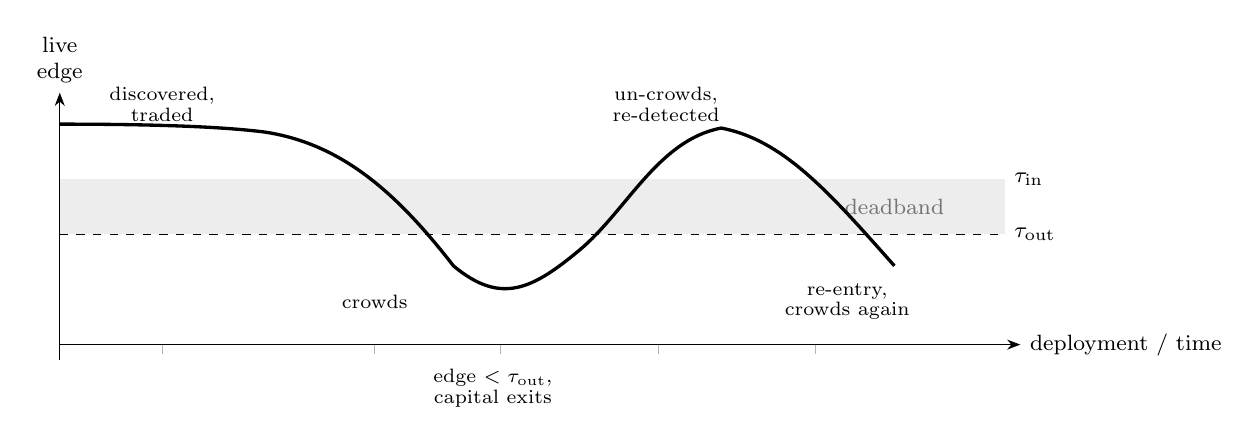
\begin{tikzpicture}[>=Stealth, font=\footnotesize]
  % axes
  \draw[->] (0,0) -- (12.2,0) node[right]{deployment / time};
  \draw[->] (0,-0.2) -- (0,3.2) node[above, align=center]{live\\ edge};
  % entry and exit threshold lines
  \draw[dashed] (0,2.1) -- (12,2.1) node[right]{$\tau_{\mathrm{in}}$};
  \draw[dashed] (0,1.4) -- (12,1.4) node[right]{$\tau_{\mathrm{out}}$};
  \fill[black!7] (0,1.4) rectangle (12,2.1);
  \node[black!55] at (10.6,1.75) {deadband};
  % the edge path: discovered high, crowded down below exit, withdraws, revives, re-enters
  \draw[very thick]
    (0,2.8) .. controls (1.5,2.8) and (2.2,2.75) .. (2.6,2.7)  % discovered, traded
    .. controls (3.6,2.55) and (4.3,1.9) .. (5.0,1.0)          % crowds below exit
    .. controls (5.6,0.5) and (6.0,0.7) .. (6.6,1.2)           % capital withdraws, un-crowds
    .. controls (7.2,1.7) and (7.6,2.6) .. (8.4,2.75)          % revives above entry
    .. controls (9.2,2.6) and (9.8,1.9) .. (10.6,1.0);         % re-entered, crowds again
  % phase markers
  \foreach \x/\lab in {1.3/discovered, 4.0/{crowding}, 5.6/{exit\,\&\,withdrawal}, 7.6/{revival}, 9.6/{re-entry}} {
    \draw[black!30] (\x,0) -- (\x,-0.12);
  }
  \node[align=center] at (1.3,3.05) {\scriptsize discovered,\\[-2pt]\scriptsize traded};
  \node[align=center] at (4.0,0.55) {\scriptsize crowds};
  \node[align=center] at (5.5,-0.55) {\scriptsize edge $<\tau_{\mathrm{out}}$,\\[-2pt]\scriptsize capital exits};
  \node[align=center] at (7.7,3.05) {\scriptsize un-crowds,\\[-2pt]\scriptsize re-detected};
  \node[align=center] at (10.0,0.55) {\scriptsize re-entry,\\[-2pt]\scriptsize crowds again};
\end{tikzpicture}
\caption{Illustrative life of one published anomaly under the deployment loop (regime~II of Theorem~\ref{thm:dichotomy}). The detected edge is traded, crowds below the exit threshold $\tau_{\mathrm{out}}$, the capital withdraws so the edge un-crowds, it is re-detected above the entry threshold $\tau_{\mathrm{in}}$, and the rule re-enters, repeating the cycle. The figure illustrates the mechanism; it is not a claim about the path of any particular signal.}
\label{fig:timeline}
\end{figure}

The two-graph model cannot exceed period two, and a longer cycle requires several signals competing for the same capacity. Rather than posit a cyclic order, we specify a crowding matrix and derive which periods can occur. Let there be $K$ signals with un-crowded edges $\mu_i$, and let deploying capital $w_j$ on signal $j$ reduce every edge through a nonnegative crowding matrix $A=(A_{ij})$,
\begin{equation}\label{eq:crossmatrix}
e_i(w)=\mu_i-\sum_{j=1}^{K}A_{ij}\,w_j,
\end{equation}
where $A_{ii}$ is self-crowding and $A_{ij}$ for $j\neq i$ is the cross-crowding that deploying $j$ imposes on $i$ through shared positions. The discovered graph records the set of signals whose edge clears the entry threshold, $\Dop$ selects active signals by the deadband applied coordinatewise, and deploying a graph commits unit capital to each active signal. The structure of $A$ controls the attainable dynamics. For part~(iii) below, let $G_i$ denote the graph with exactly signal $i$ active, and let $\Gcal_{\mathrm{sing}}=\{G_1,\dots,G_K\}$ be the singleton-active subset; the sufficient condition is stated on this subset, and if graphs with several active signals are admissible the sign conditions must in addition rule out every non-successor signal crossing the entry threshold.

\begin{theorem}[Cross-crowding and cycle length]\label{thm:multisignal}
Consider the linear coordinatewise crowding model \eqref{eq:crossmatrix}, in which unit capital is committed to each active signal, edges are linear in deployed capital, and discovery applies the deadband to each signal separately. Within this model:
\begin{enumerate}
\item[(i)] \emph{Diagonal crowding gives no long cycles.} If $A$ is diagonal, the signals are independent, each runs the one-signal phase diagram of Theorem~\ref{thm:dichotomy} separately, and every orbit is a product of fixed points and two-cycles; no coordinate has period greater than two and no cross-signal rotation occurs.
\item[(ii)] \emph{Longer cycles require cross-crowding.} Within the linear coordinatewise model, any orbit whose active-signal identity has period greater than two requires an off-diagonal crowding term: some $A_{ij}\neq0$ with $j\neq i$.
\item[(iii)] \emph{Sufficient condition for a singleton $K$-cycle.} Let $G_i$ denote the graph with exactly signal $i$ active. Suppose that after deploying $G_i$, exactly the successor signal $\sigma(i)=i+1\pmod K$ clears the entry threshold, signal $i$ falls below the exit threshold, and every other signal remains below entry. Then the singleton-active subset $\Gcal_{\mathrm{sing}}$ is invariant, $\Sbeta(G_i)=G_{\sigma(i)}$, and the orbit on $\Gcal_{\mathrm{sing}}$ has period $K$ with no fixed point.
\end{enumerate}
\end{theorem}

\begin{proof}
For (i), a diagonal $A$ makes $e_i$ depend only on $w_i$, so the update of each signal's active bit depends only on that signal's own deployed state; the joint map is the product of $K$ independent one-signal maps, each constant or a transposition by Theorem~\ref{thm:dichotomy}, so each coordinate is fixed or alternates and no coordinate has period above two. Statement (ii) is the contrapositive within this model: if $A$ were diagonal, (i) would bound every coordinate period at two, so a period above two forces an off-diagonal entry. For (iii), the stated sign conditions make, after deploying the graph $G_i$ whose single active signal is $i$, exactly one signal clear the entry threshold, namely $\sigma(i)$, while $i$ has fallen below exit and the rest remain below entry; the coordinatewise rule returns $G_{\sigma(i)}$, which is again singleton-active, so $\Gcal_{\mathrm{sing}}$ is invariant, $\Sbeta(G_i)=G_{\sigma(i)}$, and $\sigma$ is the $K$-cycle with a single orbit of period $K$ and no fixed point.
\end{proof}

Part (ii) is a statement about this linear coordinatewise model, not a universal one. Other forms of state dependence, nonlinear capital allocation, risk or funding constraints, switching costs, delayed impact, or asymmetric thresholds, can also generate longer cycles without an off-diagonal crowding term, and we do not rule them out. What the model isolates is one clean mechanism: when crowding is purely own-signal, the system can only stall or alternate, and a rotation among distinct strategies requires that deploying one signal change the detectability of another, which shared positions and capacity competition produce. The earlier period-three rotation is the case $K=3$ of part (iii), obtained from the crowding matrix rather than assumed. Proposition~\ref{prop:periodic} bounds the period of any orbit by the number of graphs; parts (i)--(iii) say which matrices realise which periods inside this model.

\begin{figure}[t]
\centering
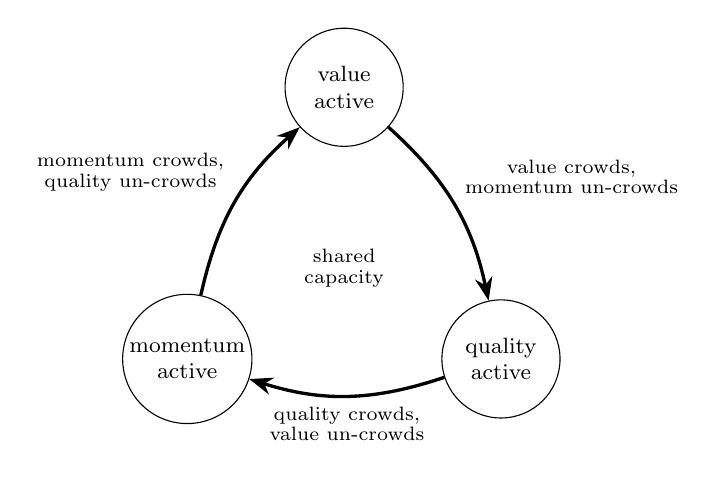
\begin{tikzpicture}[>=Stealth, font=\footnotesize,
  st/.style={draw, circle, minimum size=15mm, align=center, inner sep=1pt}]
  \node[st] (v) at (90:2.3) {value\\ active};
  \node[st] (m) at (210:2.3) {momentum\\ active};
  \node[st] (q) at (330:2.3) {quality\\ active};
  \draw[->, very thick, bend left=18] (v) to node[above right, align=center]{\scriptsize value crowds,\\[-2pt]\scriptsize momentum un-crowds} (q);
  \draw[->, very thick, bend left=18] (q) to node[below, align=center]{\scriptsize quality crowds,\\[-2pt]\scriptsize value un-crowds} (m);
  \draw[->, very thick, bend left=18] (m) to node[above left, align=center]{\scriptsize momentum crowds,\\[-2pt]\scriptsize quality un-crowds} (v);
  \node[align=center] at (0,0) {\scriptsize shared\\[-2pt]\scriptsize capacity};
\end{tikzpicture}
\caption{Illustrative three-signal rotation under cross-crowding (Theorem~\ref{thm:multisignal}(iii)). Capital concentrated in one style crowds its own edge below the exit threshold while a competing style, not currently traded, un-crowds above the entry threshold, so the deployed graph rotates value $\to$ quality $\to$ momentum $\to$ value. The rotation requires off-diagonal crowding, that is, shared positions across styles; the labels are illustrative and not a claim that these particular styles rotate in this order in any market.}
\label{fig:rotation}
\end{figure}

\begin{figure}[t]
\centering
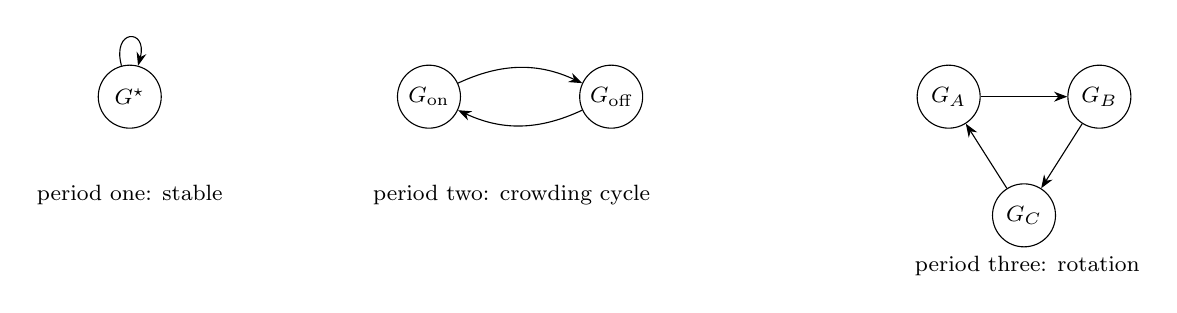
\begin{tikzpicture}[>=Stealth, every node/.style={font=\footnotesize}, st/.style={draw, circle, minimum size=8mm, inner sep=1pt}]
  \begin{scope}
    \node[st] (a1) {$G^\star$};
    \draw[->] (a1) edge[loop above, looseness=6] (a1);
    \node at (0,-1.25) {period one: stable};
  \end{scope}
  \begin{scope}[xshift=38mm]
    \node[st] (on) {$G_{\text{on}}$};
    \node[st, right=15mm of on] (off) {$G_{\text{off}}$};
    \draw[->] (on) to[bend left=25] (off);
    \draw[->] (off) to[bend left=25] (on);
    \node at (1.05,-1.25) {period two: crowding cycle};
  \end{scope}
  \begin{scope}[xshift=104mm]
    \node[st] (A) {$G_A$};
    \node[st, right=11mm of A] (B) {$G_B$};
    \node[st, below=11mm of $(A)!0.5!(B)$] (C) {$G_C$};
    \draw[->] (A) -- (B); \draw[->] (B) -- (C); \draw[->] (C) -- (A);
    \node at (1.0,-2.15) {period three: rotation};
  \end{scope}
\end{tikzpicture}
\caption{The three orbit structures the deployment scale can produce. Below the crossing scale the orbit is a fixed point. Above it, two competing graphs give the crowding two-cycle, and three competing signals under shared capacity give a rotation.}
\label{fig:orbits}
\end{figure}

\section{Finite-sample recovery}\label{sec:finitesample}

The results so far concern the population operator $\Dop$, which reads the exact law. In practice one estimates the edge statistic from a finite sample of the deployed law and applies $\Dhat_n$, and the question is whether the estimated loop follows the population loop. It does, with high probability, whenever the population edge is separated from the thresholds by more than the estimation error, which is the role the deadband margin plays.

The recovery theorem applies away from switching surfaces. It does not resolve branch selection inside the deadband, where the population margin is zero and finite-sample noise can move the estimated loop onto a different branch; inside the deadband the relevant object is a branch-selection probability, given separately in Remark~\ref{prop:branch}, not exact path recovery.

\begin{theorem}[High-probability recovery]\label{thm:finitesample}
Suppose each estimated edge statistic $\hat\phi_{j,n}$ concentrates around its population value, uniformly over reachable laws, in the sense that for each reachable law $P$, every $\epsilon>0$, and every $j=1,\dots,N_{\mathrm{edge}}$,
\begin{equation}\label{eq:concentration}
\Pr\!\big(|\hat\phi_{j,n}(P)-\phi_j(P)|>\epsilon\big)\le 2\exp(-c\,n\,\epsilon^2)
\end{equation}
for a constant $c>0$. For a state $(P,G)$ whose edge statistics clear every relevant threshold strictly, let the per-round margin be
\[
m(P,G)=\min_{j}\,\min\big(|\phi_j(P)-\tau_{\mathrm{in}}|,\ |\phi_j(P)-\tau_{\mathrm{out}}|\big),
\]
the smallest distance, over the edges discovery evaluates at this state, from an edge statistic to the nearer threshold. Along a population orbit $G_0,G_1,\dots$ write $m_t=m(\Pidep(G_t),G_t)$ and $m_{\min}=\min_{t<T}m_t$, and assume $m_{\min}>0$, that is, no visited state sits in a deadband. Then the estimated update agrees with the population update at round $t$ with probability at least $1-2N_{\mathrm{edge}}\exp(-c\,n\,m_t^2)$, where $N_{\mathrm{edge}}$ is the number of edge statistics evaluated, and over $T$ rounds
\begin{equation}\label{eq:Tbound}
\Pr\big(\hat G_t=G_t\ \text{for all }t\le T\big)\ \ge\ 1-2T\,N_{\mathrm{edge}}\exp(-c\,n\,m_{\min}^2).
\end{equation}
In particular the estimated orbit coincides with the population orbit, and exhibits the same regime, with probability approaching one as the sample grows; the transition blurs only within a band of width of order $n^{-1/2}$ around the crossing scales, where some $m_t$ approaches zero.
\end{theorem}

\begin{proof}
At a state with margin $m_t>0$, each edge statistic $\phi_j$ lies at distance at least $m_t$ from the nearer threshold, so the estimated call on edge $j$ differs from the population call only if $\hat\phi_{j,n}$ moves it across, which requires $|\hat\phi_{j,n}-\phi_j|>m_t$ and by \eqref{eq:concentration} has probability at most $2\exp(-c\,n\,m_t^2)$. A union bound over the $N_{\mathrm{edge}}$ edge statistics evaluated at the state gives the per-round bound; since discovery is a function of the resulting calls, matching all calls matches the update. The multi-round statement is inductive. Suppose the estimated and population orbits agree up to time $t$. Then the sample at round $t$ is drawn from the same deployed law $\Pidep(G_t)$ as in the population orbit, so the per-round concentration bound applies at that state; on the event that all edge calls match, the estimated update equals the population update and the orbits agree at time $t+1$. The failure event over $T$ rounds is a union of $T$ per-round failures, each at most $2N_{\mathrm{edge}}\exp(-c\,n\,m_{\min}^2)$, giving \eqref{eq:Tbound}. Setting the exponent to a constant gives a margin of order $n^{-1/2}$, hence a transition band of that width. The bound is vacuous when some visited state lies in a deadband, where $m_t=0$; this is the state-dependent case in which estimation can move the system onto a different branch, and is excluded by the assumption $m_{\min}>0$.
\end{proof}

The concentration inequality is stated abstractly because its form depends on the estimator and sampling design. For bounded or winsorised payoffs and independent samples it follows from Hoeffding-type bounds. For weakly dependent returns it may be replaced by a mixing or martingale concentration bound, with an effective sample size replacing $n$. The theorem uses only the stated deviation inequality.

Inside the deadband the population margin is zero and the theorem is silent. There the relevant object is the probability of each branch, which for a scalar statistic takes an explicit asymptotic form.

\begin{remark}[Finite-sample branch probability inside the deadband]\label{prop:branch}
Suppose a scalar edge statistic satisfies $\hat\phi_n(P)=\phi(P)+\sigma(P)n^{-1/2}Z_n$ with $Z_n\Rightarrow N(0,1)$, and $\phi(P)\in[\tau_{\mathrm{out}},\tau_{\mathrm{in}}]$. Then the normal approximation gives
\[
\Pr(\hat\phi_n>\tau_{\mathrm{in}})\approx 1-\Phi\!\left(\frac{\sqrt n\,(\tau_{\mathrm{in}}-\phi(P))}{\sigma(P)}\right),
\]
and
\[
\Pr(\hat\phi_n<\tau_{\mathrm{out}})\approx \Phi\!\left(\frac{\sqrt n\,(\tau_{\mathrm{out}}-\phi(P))}{\sigma(P)}\right).
\]
Inside the band finite samples randomise branch selection, while outside the band the error probability decays according to the estimator's deviation rate.
\end{remark}

The Monte Carlo study of the next section is a finite-sample diagnostic of the population mechanism. Since the data-generating process implements the model, the simulations do not independently validate the mechanism; they measure how estimation noise widens and shifts the transition relative to the population boundary, by a band of order $n^{-1/2}$, and biases the empirical switch scale upward as a noisy estimator predicts. The retention band is where this matters most: a state inside it has $m_t=0$, so Remark~\ref{prop:branch} rather than the recovery theorem governs the call, which is the finite-sample face of path dependence.

\section{Experiments}\label{sec:experiments}

The theory is exact for the population operator, while any application uses the finite-sample estimator, so the experiments are a finite-sample diagnostic of the population mechanism. Since the data-generating process implements the model, they do not independently validate the mechanism; they measure how far estimation noise displaces the transition from its population value. All experiments use synthetic data in which the un-crowded edge, the impact function and the detection threshold are known, so the crossing scale, the phase boundary and the cycle are known in advance and can be compared with what the estimator recovers. Every Monte Carlo fraction is reported with a ninety-five percent Wilson interval, and the population operator and the estimator are implemented separately so that the two are never conflated. The baseline parameters are collected in Table~\ref{tab:params}.

\begin{table}[h]
\centering
\begin{tabular}{lll}
\toprule
Parameter & Meaning & Baseline value \\
\midrule
$\mu$ & un-crowded edge & $0.020$ \\
$\lambda$ & linear impact coefficient & $1.0$ \\
$\tau$ & detection threshold & $0.012$ \\
$\rho$ & deadband half-width & varies \\
$\sigma$ & return noise & $0.05$ \\
$n$ & sample size per estimate & $1500$ \\
$\beta_c$ & crossing scale & $(\mu-\tau+\rho)/\lambda$ \\
\bottomrule
\end{tabular}
\caption{Baseline simulation parameters for the one-signal discovery loop.}
\label{tab:params}
\end{table}

We begin with a single signal whose un-crowded edge is $0.020$, with unit impact, detection threshold $0.012$, and per-period return noise $0.05$. The estimator forms the edge from fifteen hundred observations of the deployed law and applies strict thresholding, and the closed-form crossing scale is $0.008$. For each deployment scale we run the orbit from both starting graphs over two hundred seeds and classify the tail of each orbit as a fixed point or a two-cycle. Figure~\ref{fig:dichotomy}(a) plots the fraction of orbits that cycle, and the smallest scale at which a majority cycle is $0.008$, equal to the closed-form value at the resolution of the grid. The deployed edge moves deterministically with scale while the estimator is unbiased for the edge, so estimation noise widens the transition region without moving its centre at this sample size.

Introducing the deadband makes the detection margin explicit and lets us trace its effect. A wider margin should enlarge the stable region, and the crowding algebra of Example~\ref{ex:cycle} predicts that the boundary scale rises linearly with the margin as $\beta_c(\rho_\Dop)=(\mu-\tau+\rho_\Dop)/\lambda$. Figure~\ref{fig:dichotomy}(b) shows the cycle fraction over the plane of deployment scale and detection margin with the predicted boundary drawn on top, and the empirical frontier between the stable and cycling regions coincides with the predicted line, confirming both the sign and the slope of the dependence.

\begin{figure}[t]
\centering
\includegraphics[width=0.48\textwidth]{fig1_dichotomy.pdf}\hfill

\includegraphics[width=0.50\textwidth]{fig2_phase.pdf}
\caption{Threshold and phase boundary under finite-sample discovery. Panel (a) shows the fraction of re-discovery orbits that settle into a two-cycle as a function of deployment scale. Panel (b) shows the cycle fraction over the plane of deployment scale and detection margin. In both panels the dashed or solid line is the population crossing scale $\beta_c(\rho_\Dop)=(\mu-\tau+\rho_\Dop)/\lambda$; the smooth transition around it is finite-sample uncertainty in the estimated discovery rule, not a population feature.}
\label{fig:dichotomy}
\end{figure}

We then vary the conditions under which the threshold is recovered. Table~\ref{tab:robust} reports the empirical switch scale against the model-implied crossing scale as the sample size, the return noise, the detection threshold, the entry and exit margins, and the curvature of the impact function are changed in turn. As the sample grows the switch scale falls towards the crossing scale, approaching it from above because a noisier edge estimate keeps the deadband from flipping until crowding is slightly deeper, so that small samples bias the threshold upward in the direction the estimator predicts. The error grows gracefully with return noise, from one grid step at the lowest noise level to about three grid steps at the highest. The threshold moves with the detection threshold and with the exit margin exactly as the expression $(\mu-\tau+\rho)/\lambda$ requires, and the two-regime split persists when impact is concave rather than linear, with the crossing scale at the value the square-root impact model implies. Figure~\ref{fig:robust}(a) shows the headline curve with its confidence band, and Figure~\ref{fig:robust}(b) plots the empirical switch scale against the predicted crossing scale across the whole battery, with the points lying on the identity line and the small-sample cases sitting just above it.

\begin{table}[t]
\centering
\small
\begin{tabular}{llcc}
\toprule
Variation & Setting & Predicted $\beta_c$ & Empirical switch \\
\midrule
Sample size $T$ & $250$ & $0.008$ & $0.0095$ \\
                & $500$ & $0.008$ & $0.0090$ \\
                & $1{,}500$ & $0.008$ & $0.0085$ \\
                & $5{,}000$ & $0.008$ & $0.0085$ \\
\addlinespace
Return noise $\sigma$ & $0.02$ & $0.008$ & $0.0085$ \\
                      & $0.10$ & $0.008$ & $0.0090$ \\
                      & $0.20$ & $0.008$ & $0.0110$ \\
\addlinespace
Threshold $\tau$ & $0.008$ & $0.012$ & $0.0125$ \\
                 & $0.016$ & $0.004$ & $0.0045$ \\
\addlinespace
Asymmetric $(\rho_{\mathrm{in}},\rho_{\mathrm{out}})$ & $(0.004,0.001)$ & $0.009$ & $0.0095$ \\
                 & $(0.001,0.004)$ & $0.012$ & $0.0130$ \\
\addlinespace
Concave impact & $\lambda=0.5$ & $0.000256$ & $0.000287$ \\
               & $\lambda=1.0$ & $0.000064$ & $0.000078$ \\
\bottomrule
\end{tabular}
\caption{Empirical switch scale against the model-implied crossing scale across the robustness battery. The grid resolution is $0.0005$ for the linear panels and is refined to resolve the smaller crossing scale under concave impact. The switch scale exceeds the crossing scale by at most a few grid steps and approaches it as the sample grows, and the gap widens with return noise as a finite-sample estimator predicts.}
\label{tab:robust}
\end{table}

\begin{figure}[t]
\centering

\includegraphics[width=0.99\textwidth]{fig4_robust.pdf}
\caption{Robustness of the threshold. Panel (a) shows the cycle fraction with a ninety-five percent Wilson band, which is narrow and crosses one-half at the crossing scale. Panel (b) shows the empirical switch scale against the predicted crossing scale across the battery, with the points on the identity line and the small-sample cases slightly above it.}
\label{fig:robust}
\end{figure}

Two further experiments display the structure of the transition directly. The first is the bifurcation diagram of the live edge, which is the dynamical-systems counterpart of the regime schematic. For each deployment scale we run the loop to its long-run regime and record the distinct values of the live edge that the orbit visits in its tail. Figure~\ref{fig:bifurcation} shows the result. Below the crossing scale the tail visits a single value, the surviving edge, which declines with scale along one branch. At the crossing scale the branch splits, and above it the orbit visits two values, the un-crowded edge when capital is withdrawn and the crowded edge when it is deployed, the second declining towards zero as scale grows. The picture makes the period-one to period-two transition visible in an observable quantity rather than in the abstract graph label.

\begin{figure}[t]
\centering

\includegraphics[width=0.52\textwidth]{fig5_bifurcation.pdf}
\caption{Bifurcation of the live edge. Below the crossing scale the long-run orbit visits a single live-edge value, the surviving edge, which falls with scale. Above the crossing scale the orbit visits two values, the un-crowded edge and the crowded edge, the signature of the two-cycle.}
\label{fig:bifurcation}
\end{figure}

The second experiment measures how long the loop takes to settle and which period it settles into. Theorem~\ref{thm:threshold} states that below the crossing scale the map is constant on the reachable set, so the orbit should reach the stable graph in a single step. Figure~\ref{fig:transient}(a) confirms that the mean transient is close to zero throughout the stable region and again throughout the cycling region, with a peak at the crossing scale. Transient length increases near the threshold because the surviving edge sits inside the detection band for several rounds before the noise resolves the call, while it remains short away from the boundary. Figure~\ref{fig:transient}(b) shows the fraction of orbits that realise each period, with a clean switch from period one to period two at the crossing scale and a thin band of unresolved orbits in between. Across the stable region almost every orbit is a fixed point reached in about two steps, and across the cycling region almost every orbit is a two-cycle, so the population statements of Section~\ref{sec:theory} survive estimation with only a narrow transitional band.

\begin{figure}[t]
\centering

\includegraphics[width=0.99\textwidth]{fig6_transient.pdf}
\caption{Convergence and realised period under finite-sample discovery. Panel (a) shows the mean transient length, near zero away from the population crossing scale and rising near it as finite samples blur branch selection. Panel (b) shows the fraction of orbits realising period one and period two, switching at the population crossing scale.}
\label{fig:transient}
\end{figure}

The last experiment embeds the mechanism in a cross-section. The following cross-sectional panel is a mechanism check, not a realistic market simulator. Before reporting it we make the capacity model explicit, because the closed-form benchmarks it produces are stated nowhere else and a reader should not have to recover them from the code. An asset has un-crowded momentum decile-spread edge $\mu_0$. An allocator deploys aggregate capital $w\ge0$, which crowds the spread linearly to $\mu_0-\lambda w$, and chooses $w$ by mean--variance preferences, maximising the certainty-equivalent
\begin{equation}\label{eq:capacity}
U(w)=\mu_0\,w-\tfrac12(\lambda+\kappa)\,w^2,
\end{equation}
where $\lambda$ is the impact coefficient of Example~\ref{ex:cycle} and $\kappa>0$ is the risk-aversion coefficient, the marginal cost of capital we vary in the experiment. The first-order condition $\mu_0-(\lambda+\kappa)w=0$ gives the performatively stable crowd and the surviving edge in closed form,
\begin{equation}\label{eq:wps}
w_{\mathrm{PS}}=\frac{\mu_0}{\lambda+\kappa},\qquad
e_{\mathrm{PS}}=\mu_0-\lambda w_{\mathrm{PS}}=\frac{\kappa\,\mu_0}{\lambda+\kappa},
\end{equation}
and the discovery cycle of Theorem~\ref{thm:dichotomy} appears once the deployed edge $\mu_0-\lambda\beta$ is driven below the lower detection band, at the crossing scale $\beta_c=(\mu_0-\tau+\rho)/\lambda$ of Example~\ref{ex:cycle}. The experiment uses $\mu_0=0.018$ per month, impact $\lambda=0.9$, risk aversion $\kappa=1.0$, detection threshold $\tau=0.010$, and detection margin $\rho=0.004$, with the edge estimated from a window long enough that the deadband rather than estimation noise governs the flips. Equation~\eqref{eq:wps} then gives $w_{\mathrm{PS}}=e_{\mathrm{PS}}=0.0095$, equal because $\lambda$ and $\kappa$ are close, and \eqref{eq:capacity}'s crossing scale is $\beta_c=0.0133$. Figure~\ref{fig:momentum}(c) shows the deployed-graph orbit below and above the crossing scale; at the lower scale the strategy is deployed in every round and the edge survives, while at the higher scale the deployed graph alternates. Figure~\ref{fig:momentum}(d) shows the average live edge falling with scale and flattening at the detection threshold near the crossing scale. The deployed fraction above the crossing scale is not exactly one half because of the initial transient and because re-entry from the inactive graph always succeeds while exit requires the surviving edge to cross the full deadband, so we read it as evidence of alternation rather than as an estimate of the cycle's duty ratio. We present this panel as evidence that the two-graph mechanism survives embedding in a cross-section, and not as a realistic simulation of a market.

\begin{figure}[t]
\centering

\includegraphics[width=0.99\textwidth]{fig3_momentum.pdf}
\caption{The crowding cycle in a simulated momentum panel. Panel (c) shows the deployed-graph orbit below the crossing scale, a fixed point, and above it, a two-cycle. Panel (d) shows the average live edge as a function of deployment scale, with the detection threshold and the crossing scale marked, falling towards the threshold as scale rises.}
\label{fig:momentum}
\end{figure}

\FloatBarrier
\section{Evidence from published anomalies}\label{sec:empirical}

The theory makes two empirical predictions that public data can examine separately. The decay prediction is that deployment erodes a discovered edge once the signal is detected and traded, so the surviving edge after wide deployment is below its un-crowded level. The cycle prediction is that the erosion is not monotone: above a crowding scale the system enters the two-cycle of Theorem~\ref{thm:dichotomy}, in which a heavily crowded edge later reverts. Both tests concern the deployment dynamics of an estimated edge, which is what the theory describes, and we return at the end of the section to what they do not establish.

\paragraph{Decay.}
This subsection is not a new anomaly-decay result. It verifies that the public data used here reproduce the known post-publication attenuation documented in the literature, and uses that attenuation as the first ingredient required by the deployment mechanism. We use the Open Source Asset Pricing data of \citet{chen2020}, which provide monthly long-short returns for $212$ published cross-sectional predictors together with each predictor's in-sample period and publication year. For each predictor we take its long-short decile return series, measure the average monthly edge in the original in-sample window and again in the post-publication window, and pair the two within predictor, weighting predictors equally and dropping those with fewer than twenty-four months in either window. The mean in-sample edge is $0.62\%$ per month and the mean post-publication edge is $0.30\%$ per month, an absolute decline of $0.32$ percentage points, just over half ($52\%$) of the original edge, with a paired $t$-statistic of $7.8$ across the $210$ predictors with a positive in-sample edge ($p<10^{-12}$); the median decline is $0.32$ percentage points, close to the mean, so the result is not driven by a few large outliers. To check that it is not an artifact of unequal post-publication sample lengths, we repeat the calculation using fixed post-publication windows of five and ten years where available: the mean decline is $0.30$ percentage points ($48\%$ of in-sample, $t=6.5$) at five years and $0.30$ percentage points ($48\%$, $t=7.6$) at ten years, with medians of $0.25$ and $0.26$ percentage points, so the attenuation is materially unchanged. The magnitude matches the post-publication attenuation reported by \citet{mclean2016}. As a falsification check we repeat the exercise on the $114$ placebo signals supplied with the same data, characteristics constructed to have no genuine predictive content. Because placebos have no publication date, we split each placebo's own sample at its midpoint as a pseudo-event and compare the two halves, mirroring the predictor test. The placebos show essentially no decline: a mean change of $0.05$ percentage points and a median of $0.02$, against $0.32$ for the published predictors, with a $t$-statistic of $1.9$ that is at most marginal. The contrast between a $52\%$ attenuation in published signals and a near-zero change in placebos is the form the mechanism predicts, since only genuinely traded edges are crowded. Publication is an imperfect proxy for the onset of heavy deployment, since it may coincide with data-mining correction, changing market structure, or declining mispricing; we use it because it is observable and dated, not because it equals deployed capital. Figure~\ref{fig:decay} shows the average edge in event time relative to publication for predictors and placebos, and Table~\ref{tab:decay} collects the decline across window definitions.

\begin{table}[h]
\centering
\begin{tabular}{lccccc}
\toprule
Sample / window & $n$ & in-sample & post-pub & mean decline & median \\
 & & (\%/mo) & (\%/mo) & (pp, \% of IS) & (pp) \\
\midrule
Predictors, full post & $210$ & $0.62$ & $0.30$ & $0.32$ ($52\%$), $t{=}7.8$ & $0.32$ \\
Predictors, 5-year post & $210$ & $0.62$ & $0.33$ & $0.30$ ($48\%$), $t{=}6.5$ & $0.25$ \\
Predictors, 10-year post & $210$ & $0.62$ & $0.32$ & $0.30$ ($48\%$), $t{=}7.6$ & $0.26$ \\
Placebos, split at midpoint & $114$ & --- & --- & $0.05$, $t{=}1.9$ & $0.02$ \\
\bottomrule
\end{tabular}
\caption{Post-publication decay in the Open Source Asset Pricing data. Published predictors lose about half their in-sample edge across all window definitions; placebo signals show a near-zero, at most marginal change.}
\label{tab:decay}
\end{table}

\paragraph{Cycle.}
The cycle prediction concerns the deployment scale, which the decay test does not observe directly. We therefore turn to a price-based proxy for arbitrage crowding. Following \citet{lou2022}, we measure comomentum as the average pairwise correlation of daily returns among the stocks a momentum strategy holds, computed within the winner and loser deciles over the formation window and then averaged. We form momentum deciles each month by the standard twelve-minus-one cumulative return, skipping the most recent month, on a universe restricted to common shares priced above five dollars among the most liquid names by dollar volume. The liquidity screen is applied using information available at the formation date; the public Stooq universe may still differ from a fully point-in-time CRSP universe with delisting returns and historical share-code filters. Comomentum is computed from daily returns within the formation window only, using the months strictly before each forward return window, so the proxy never overlaps the returns it predicts. We construct the series from daily U.S. equity returns over $1990$--$2025$, yielding $424$ monthly observations of comomentum ranging from $0.06$ to $0.50$. We interpret comomentum as a price-based proxy for deployment pressure, following \citet{lou2022}, not as an observed capital-flow measure; it may also load on volatility, liquidity, or common factor shocks, which the sort does not separate out. The Stooq implementation is used for public reproducibility; a CRSP replication would be the institutional benchmark because it handles delisting returns and standard share-code filters more directly, so we read the comomentum exercise as public-data consistency evidence rather than a final asset-pricing estimate.

The theory predicts that returns should behave differently at low and high deployment: where the proxy is low the strategy should resemble the stable regime and its edge persist, while where it is high the strategy should resemble the cycling regime and its edge revert. Sorting months into quintiles of comomentum and measuring the subsequent momentum return shows this pattern. In the lowest comomentum quintile the forward twelve-month momentum return is flat at $+0.02\%$ per month; it falls monotonically across quintiles to $-2.06\%$ per month in the highest. The difference between the extreme quintiles is $-2.08\%$ per month at the twelve-month horizon and $-1.82\%$ per month at twenty-four months. Because the forward returns overlap, we compute $t$-statistics with Newey--West standard errors at lags matching the holding horizon; the high-minus-low differences are significant at both horizons ($t=-4.4$ and $t=-4.7$). This reproduces the destabilisation \citet{lou2022} document. We do not control for factor or risk exposure, so the sort is a conditional-return pattern consistent with the crowding mechanism rather than a structural identification of it. As robustness, the forward momentum return can be regressed on the comomentum quintile while controlling for market volatility, market return, aggregate liquidity, momentum-crash indicators, and standard factor returns,
\[
R^{\mathrm{mom}}_{t:t+h}=\alpha+b\,Q^{\mathrm{comom}}_t+\gamma^\top Z_t+\varepsilon_{t+h},
\]
with inference based on Newey--West or block-bootstrap standard errors at lags matching the holding horizon $h$, since the forward returns overlap. We include the specification to state the required next robustness check; it is not estimated in the present public-data exercise. We do not claim the comomentum sort is a structural estimate. Figure~\ref{fig:phase}(b) shows the monotone decline of the forward edge across comomentum quintiles, and Figure~\ref{fig:phase}(a) shows the comomentum series.

The comomentum sort gives a continuous crowding axis with $424$ months of resolution, along which the conditional forward return moves from flat to sharply reverting. We emphasise what this does and does not show. It does not observe the graph-level loop $G_{\mathrm{on}}\to G_{\mathrm{off}}\to G_{\mathrm{on}}$, does not estimate the thresholds or the impact coefficient, and does not exhibit alternation in the rediscovered status of a strategy; it is a conditional-return pattern sorted by a crowding proxy, not a measurement of the cycle in graph space. What it provides is evidence consistent with the second ingredient of the mechanism, that high deployment is associated with reversal, alongside the first ingredient established by the decay test.

\begin{figure}[t]
\centering
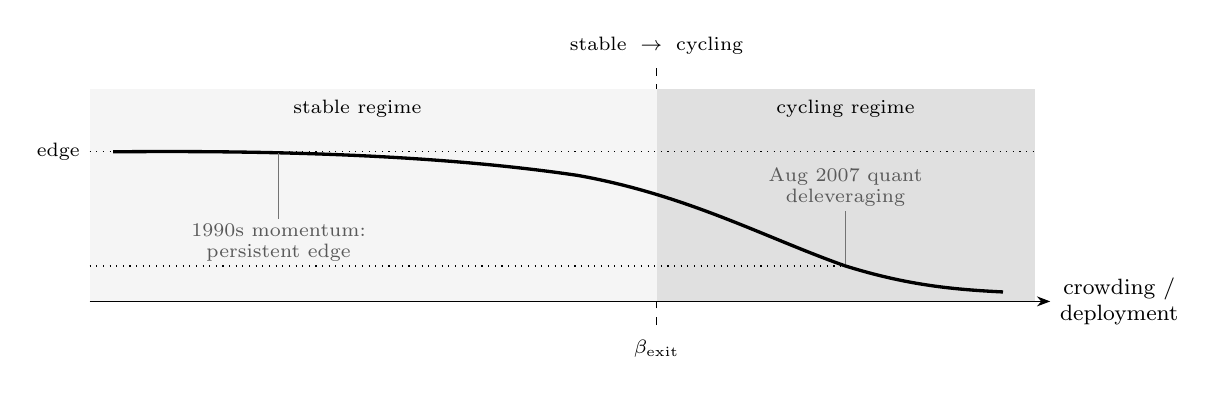
\begin{tikzpicture}[>=Stealth, font=\footnotesize]
  % horizontal crowding axis
  \draw[->] (0,0) -- (12.2,0) node[right, align=center]{crowding /\\ deployment};
  % regime split
  \draw[dashed] (7.2,-0.3) -- (7.2,3.0);
  \node[align=center] at (7.2,3.25) {\scriptsize stable $\;\to\;$ cycling};
  \node[align=center] at (7.2,-0.6) {\scriptsize $\beta_{\mathrm{exit}}$};
  % shaded regimes
  \fill[black!4] (0,0) rectangle (7.2,2.7);
  \fill[black!12] (7.2,0) rectangle (12,2.7);
  \node at (3.4,2.45) {\scriptsize stable regime};
  \node at (9.6,2.45) {\scriptsize cycling regime};
  % forward-return curve: flat then reverting (mirrors the quintile pattern)
  \draw[very thick]
    (0.3,1.9) .. controls (2.5,1.92) and (4.5,1.85) .. (6.2,1.6)
    .. controls (7.6,1.35) and (8.6,0.8) .. (9.6,0.45)
    .. controls (10.4,0.2) and (11.0,0.15) .. (11.6,0.12);
  \draw[dotted] (0,1.9) -- (12,1.9);
  \node[left] at (0,1.9) {\scriptsize edge};
  \draw[dotted] (0,0.45) -- (9.6,0.45);
  % example episodes
  \draw[black!55] (2.4,1.88) -- (2.4,1.05);
  \node[align=center, black!65] at (2.4,0.75) {\scriptsize 1990s momentum:\\[-2pt]\scriptsize persistent edge};
  \draw[black!55] (9.6,0.47) -- (9.6,1.15);
  \node[align=center, black!65] at (9.6,1.45) {\scriptsize Aug 2007 quant\\[-2pt]\scriptsize deleveraging};
\end{tikzpicture}
\caption{Illustrative reading of the comomentum sort against the phase diagram. Where the crowding proxy is low the forward edge is roughly flat, as for momentum through much of the 1990s; where it is high the edge reverts, the regime in which the correlated quant deleveraging of August 2007 \citep{khandani2011} sits. The placement of episodes is illustrative and is not an estimate of $\beta_{\mathrm{exit}}$ for any strategy.}
\label{fig:regimes}
\end{figure}

\begin{figure}[t]
\centering

\includegraphics[width=0.6\textwidth]{real_fig_decay.pdf}
\caption{Post-publication decay of published anomalies. Average monthly long-short edge in event time relative to the publication year, for the $212$ predictors and for the placebo signals, from the Open Source Asset Pricing data. The predictor edge falls by just over half after publication; the placebo edge does not.}
\label{fig:decay}
\end{figure}

\begin{figure}[t]
\centering

\includegraphics[width=0.48\textwidth]{real_fig_comomentum.pdf}\hfill

\includegraphics[width=0.48\textwidth]{real_fig_phase.pdf}
\caption{Forward momentum return along a crowding proxy. Panel (a) plots comomentum, the within-decile daily-return correlation that proxies for deployed arbitrage capital, over $1990$--$2025$. Panel (b) shows the forward twelve-month momentum return by comomentum quintile: flat where the proxy is low and strongly reverting where it is high, consistent with the crowding mechanism.}
\label{fig:phase}
\end{figure}

\paragraph{What the evidence supports.}
The two tests are consistent with the two ingredients of the mechanism: the edge of a deployed signal decays once it is widely traded, and reversal is concentrated where a price-based proxy for crowding is highest. This is consistency evidence, not validation of the model. The empirical evidence should be read as ingredient-level consistency, not identification of the graph loop. A per-strategy test would require observing or instrumenting deployed capital, estimating the post-deployment edge under own and competitor flow, and separating deployment-induced cycles from exogenous regime cycles. The comomentum evidence is therefore suggestive of the crowding channel rather than a structural estimate of $\Pidep$, the impact coefficient $\lambda$, or the switching thresholds. Neither test observes the discovery loop, estimates its thresholds, or identifies deployment as an intervention; the decay test uses publication as a proxy for the onset of deployment, the cycle test uses comomentum as a proxy for deployment pressure, and neither identifies the causal graph behind a signal. These are the open requirements for turning the cross-sectional consistency shown here into a per-strategy test.

\section{Related work}\label{sec:related}

The stable graph is the discovery-level counterpart of the performatively stable model of \citet{perdomo2020}, who analyse repeated risk minimisation on a distribution that depends on the deployed decision and give a contraction condition for convergence to a stable point; the older observation that a public forecast can be self-confirming is due to \citet{grunberg1954}, and the framework has since been surveyed and extended \citep{hardt2023past, mendlerdunner2022anticipating}. The present setting differs in a way that changes the mathematics: the deployed object is a graph drawn from a finite set rather than a continuous parameter. A contraction argument is therefore unavailable, finiteness supplies the existence of an eventual regime, and a margin on the reachable set supplies the threshold. A separate line of work shows that restricting a predictor to causal features can produce performative stability without retraining \citep{kulynych2022causal}; that result removes the feedback by construction, whereas our concern is the regime in which the feedback is strong enough to destroy every stable graph and replace it with a cycle. The mechanism is also related to limits-to-arbitrage and adaptive-market views of anomaly persistence, in which capital flows, risk limits, and crowded unwinds attenuate or reverse expected returns. Our contribution is not a new equilibrium model of limits to arbitrage; it is a finite-state discovery loop showing how the act of repeatedly detecting and deploying a signal can itself generate stable or cyclic graph states. To our knowledge, the finite graph-valued discovery loop and the explicit entry--exit crowding phase diagram have not been isolated in this form, nor has the two-cycle been identified with post-publication decay and revival.

The crowding model is the minimal one of Example~\ref{ex:cycle} and Equation~\eqref{eq:capacity}: a per-unit edge that falls linearly in deployed capital, with a concave variant in Section~\ref{sec:experiments}. The linear-impact, mean--variance form is not novel and serves only to make the discovery cycle explicit; we cite the capacity literature to place the assumption, not to derive results from it. \citet{mclean2016} document that the predictability of published cross-sectional signals declines out of sample and again after publication, attributing this to informed trading; \citet{chordia2014} link the attenuation of anomalies to rising liquidity and arbitrage; and \citet{chen2020} argue that publication bias is too small to account for the post-publication decay, leaving mispricing as the operative channel. The externalities arbitrageurs impose on one another as a strategy crowds were emphasised by \citet{stein2009}, the correlated quant deleveraging of August 2007 was analysed by \citet{khandani2011}, and \citet{lou2022} infer arbitrage activity from the post-crowding correlation structure of returns, the measure our cycle test uses. Our results connect to the programme on causal portfolio construction \citep{rodriguez2023, rodriguez2025causal, rodriguez2025necessary, rodriguez2025pde} and to the filtration-relative reading of predictability of \citep{noguer2026markets}, but use none of their machinery. The contribution relative to all of this is to place the decay inside the discovery loop and to show that the scale at which the edge decays is the scale at which the stable regime gives way to the cycle.

\FloatBarrier
\section{Conclusion}\label{sec:conclusion}

A graph discovered in order to trade is one step in a system that includes its own deployment, and the long-run behaviour of that system is set by the scale at which it is deployed. In the model, deployment is an intervention, so the loop is a sequence of interventions and stability asks whether a graph is a fixed point of its own interventional consequence. Below a strictly positive scale the discovered graph is a unique fixed point on the reachable set and the edge persists; above it a stable graph need not exist and the orbit can become a crowding cycle of decay and revival, with a retention band inside the stable regime where continuation and re-entry occur at different scales. Within a linear cross-crowding model, cycles longer than two require off-diagonal crowding between signals, and away from switching surfaces the estimated loop tracks the population loop with high probability outside a transition band of order $n^{-1/2}$.

The empirical implication is not that publication or comomentum identifies the graph loop. It is that the two observable ingredients required by the loop, post-discovery decay and high-crowding reversal, are present in public data. The next step is a per-strategy deployment record: own capital, competitor crowding, post-deployment edge estimates, and switching thresholds. Only with those quantities can the model be taken from a structural explanation of decay and revival to an identified diagnostic of a live strategy. The practical reading in the meantime is concrete: if post-publication decay and the later reversion of crowded trades are two phases of one deployment-driven cycle, as the mechanism suggests and the data do not contradict, then a strategy that looks arbitraged away may be in the trough of a cycle rather than permanently dead, and a backtest that re-enters on apparent revival trades the cycle itself.

\section*{Reproducibility}\label{sec:repro}
The Monte Carlo results run from fixed seeds and are reproduced by the scripts in the replication package: \texttt{exp1\_dichotomy.py} for the threshold, \texttt{exp2\_phase.py} for the phase boundary, \texttt{exp3\_momentum.py} for the momentum panel, \texttt{exp4\_robust.py} for the robustness battery with Wilson intervals, \texttt{exp5\_bifurcation.py} for the bifurcation diagram, and \texttt{exp6\_transient.py} for the transient and period structure, with figures produced by \texttt{make\_figs.py}, \texttt{make\_fig4.py} and \texttt{make\_fig56.py}. Each script writes a summary file recording its parameters and recovered quantities, and the population operators are implemented separately from the finite-sample estimators.

The empirical results of Section~\ref{sec:empirical} are reproduced from public data by two notebooks. The decay test uses the Open Source Asset Pricing release \citep{chen2020}: \texttt{osap\_decay.ipynb} reads the long-short predictor returns, the placebo returns, and the signal documentation, partitions each predictor into its in-sample and post-publication windows, and computes the paired decline and its $t$-statistic, producing \texttt{real\_fig\_decay.pdf}. The window-robustness and placebo computations of Table~\ref{tab:decay} are reproduced by \texttt{decay\_windows.py} and \texttt{placebo\_decay.py}, which read the wide long-short return file and the placebo portfolio file directly. The cycle test uses daily U.S. equity returns: \texttt{comomentum.ipynb} forms monthly momentum deciles on the liquid universe, computes comomentum as the within-decile pairwise return correlation over the formation window following \citet{lou2022}, sorts months into comomentum quintiles, and measures the forward momentum return, producing \texttt{real\_fig\_comomentum.pdf} and \texttt{real\_fig\_phase.pdf}. Both notebooks record the sample period, the universe filters, and every reported figure. The data are redistributed by their original providers and the notebooks download them directly, so no proprietary data is included in the package. The complete replication package is archived at \url{https://doi.org/10.5281/zenodo.21038235}.

The replication package includes a requirements file, the code version hash, the random seeds, the data download dates, and a manifest mapping each table and figure to the script that produces it, summarised in Table~\ref{tab:repro}.

\begin{table}[h]
\centering
\begin{tabular}{lll}
\toprule
Output & Script/notebook & Data source \\
\midrule
Figure~\ref{fig:dichotomy} & \texttt{exp1\_dichotomy.py}, \texttt{exp2\_phase.py} & synthetic \\
Figure~\ref{fig:robust} & \texttt{exp4\_robust.py} & synthetic \\
Figure~\ref{fig:bifurcation} & \texttt{exp5\_bifurcation.py} & synthetic \\
Figure~\ref{fig:transient} & \texttt{exp6\_transient.py} & synthetic \\
Figure~\ref{fig:momentum} & \texttt{exp3\_momentum.py} & synthetic \\
Figure~\ref{fig:decay} & \texttt{osap\_decay.ipynb} & OSAP \\
Figure~\ref{fig:phase} & \texttt{comomentum.ipynb} & daily equity returns \\
\bottomrule
\end{tabular}
\caption{Replication map for figures.}
\label{tab:repro}
\end{table}

\begin{thebibliography}{99}
\bibitem[Chen and Zimmermann(2020)]{chen2020} A.~Y. Chen and T.~Zimmermann. Publication bias and the cross-section of stock returns. \emph{Review of Asset Pricing Studies}, 10(2):249--289, 2020.
\bibitem[Chickering(2002)]{chickering2002} D.~M. Chickering. Optimal structure identification with greedy search. \emph{Journal of Machine Learning Research}, 3:507--554, 2002.
\bibitem[Chordia et al.(2014)]{chordia2014} T.~Chordia, A.~Subrahmanyam, and Q.~Tong. Have capital market anomalies attenuated in the recent era of high liquidity and trading activity? \emph{Journal of Accounting and Economics}, 58(1):41--58, 2014.
\bibitem[Grunberg and Modigliani(1954)]{grunberg1954} E.~Grunberg and F.~Modigliani. The predictability of social events. \emph{Journal of Political Economy}, 62(6):465--478, 1954.
\bibitem[Hardt and Mendler-D\"unner(2023)]{hardt2023past} M.~Hardt and C.~Mendler-D\"unner. Performative prediction: Past and future. arXiv:2310.16608, 2023.
\bibitem[Khandani and Lo(2011)]{khandani2011} A.~E. Khandani and A.~W. Lo. What happened to the quants in August 2007? Evidence from factors and transactions data. \emph{Journal of Financial Markets}, 14(1):1--46, 2011.
\bibitem[Kulynych(2022)]{kulynych2022causal} B.~Kulynych. Causal prediction can induce performative stability. In \emph{ICML 2022 Workshop on Spurious Correlations, Invariance, and Stability}, 2022.
\bibitem[Lou and Polk(2022)]{lou2022} D.~Lou and C.~Polk. Comomentum: Inferring arbitrage activity from return correlations. \emph{Review of Financial Studies}, 35(7):3272--3302, 2022.
\bibitem[McLean and Pontiff(2016)]{mclean2016} R.~D. McLean and J.~Pontiff. Does academic research destroy stock return predictability? \emph{Journal of Finance}, 71(1):5--32, 2016.
\bibitem[Mendler-D\"unner et al.(2022)]{mendlerdunner2022anticipating} C.~Mendler-D\"unner, F.~Ding, and Y.~Wang. Anticipating performativity by predicting from predictions. In \emph{Advances in Neural Information Processing Systems}, 2022.
\bibitem[Noguer i Alonso(2026)]{noguer2026markets} M.~Noguer i Alonso. Markets are not random, they are hard to predict. arXiv:2606.08209, 2026.
\bibitem[Perdomo et al.(2020)]{perdomo2020} J.~C. Perdomo, T.~Zrnic, C.~Mendler-D\"unner, and M.~Hardt. Performative prediction. In \emph{Proceedings of the 37th International Conference on Machine Learning}, pages 7599--7609, 2020.
\bibitem[Rodr\'iguez Dom\'inguez(2023)]{rodriguez2023} A.~Rodr\'iguez Dom\'inguez. Portfolio optimization based on neural networks sensitivities from assets dynamics respect common drivers. \emph{Machine Learning with Applications}, 11:100447, 2023.
\bibitem[Rodr\'iguez Dom\'inguez(2025a)]{rodriguez2025causal} A.~Rodr\'iguez Dom\'inguez. Causal portfolio optimization: Principles and sensitivity-based solutions. arXiv:2504.05743, 2025.
\bibitem[Rodr\'iguez Dom\'inguez(2025b)]{rodriguez2025necessary} A.~Rodr\'iguez Dom\'inguez. Is causality necessary for efficient portfolios? A computational perspective on predictive validity and model misspecification. arXiv:2507.23138, 2025.
\bibitem[Rodr\'iguez Dom\'inguez(2025c)]{rodriguez2025pde} A.~Rodr\'iguez Dom\'inguez. Causal PDE-control for adaptive portfolio optimization under partial information. arXiv:2509.09585, 2025.
\bibitem[Spirtes et al.(2000)]{spirtes2000} P.~Spirtes, C.~Glymour, and R.~Scheines. \emph{Causation, Prediction, and Search}. MIT Press, Cambridge, MA, 2nd edition, 2000.
\bibitem[Stein(2009)]{stein2009} J.~C. Stein. Presidential address: Sophisticated investors and market efficiency. \emph{Journal of Finance}, 64(4):1517--1548, 2009.
\end{thebibliography}

\end{document}
